\documentclass{beamer}
\usepackage{graphicx}
\usepackage{verbatim}
\usepackage{alltt}
\usepackage{xcolor}
\usepackage{listings}
\usepackage{hyperref}
\setbeamertemplate{navigation symbols}{}%remove navigation symbols

\renewcommand\UrlFont{\color{blue}}

\newcommand\inputml[1]{\lstinputlisting[language={[Objective]Caml}]{#1}}

\lstdefinelanguage{OCaml}{
  keywords={
    and,as,assert,asr,begin,class,constraint,do,done,downto,effect,else,end,exception,
    external,false,for,fun,function,functor,if,implicit,in,include,inherit,initializer,
    land,lazy,let,lor,lsl,lsr,lxor,macro,match,method,mod,module,mutable,new,object,
    of,open,or,private,rec,sig,struct,then,to,true,try,type,val,virtual,when,
    with,while},
  comment=[s]{(*\ }{\ *)},
}

\definecolor{darkgreen}{rgb}{0,0.2,0}
\definecolor{darkblue}{rgb}{0.1,0.1,0.8}
\definecolor{darkbrown}{rgb}{0.5,0.3,0.0}
\definecolor{grey}{rgb}{0.5,0.5,0.5}
\definecolor{darkgrey}{rgb}{0.2,0.2,0.2}
\definecolor{highlight}{rgb}{1.0,1.0,0.4}

\lstdefinestyle{ocaml}{
  basicstyle=\ttfamily\scriptsize,
  basewidth=0.5em,
  commentstyle=\color{darkgreen},
  escapeinside={(**}{)},
  keywordstyle=\color{darkblue},
  language=OCaml,
  morekeywords={macro},
  stringstyle=\color{blue},
  showstringspaces=false,
  mathescape=true,
  moredelim=**[is][]{?}{?},
  moredelim=**[is][]{&}{&},
}

\lstdefinestyle{output}{
  basicstyle=\ttfamily\small,
  basewidth=0.5em,
}

\lstset{literate=%
{->}{{$\to$}}2
{...}{{$\ldots$}}2
}

\newcommand\mlkeyword[1]{{\ttfamily\color{darkblue} #1}}

\title[Eio]{Eio 1.0 – Effects-based IO for OCaml 5}
\author[Thomas Leonard]
{Thomas Leonard\and Patrick Ferris\and Christiano Haesbaert\and Lucas Pluvinage\and Vesa Karvonen\and Sudha Parimala\and KC Sivaramakrishnan\and Vincent Balat\and Anil Madhavapeddy}
\institute{Tarides}
\date[OCaml 2023]{The OCaml Users and Developers Workshop, Sep 2023}

\begin{document}

\definecolor{grey}{gray}{0.6}

\frame{\titlepage}

\begin{frame}
	\frametitle{Overview}
	\begin{itemize}
		\item Motivation and design
		\item Interoperability (Lwt, Async, Kcas, Domainslib)
		\item Comparison with Lwt
		\item Experiences porting software
	\end{itemize}
\end{frame}

\begin{frame}[fragile]
	\frametitle{Motivation}
	\begin{itemize}
		\item Support effects
		\begin{itemize}
			\item No difference between sequential and concurrent code
			\item No special monad syntax
			\item Can use \mlkeyword{try}, \mlkeyword{match}, \mlkeyword{while}, etc
			\item No separate Lwt or Async versions of code
			\item No heap allocations needed to simulate a stack
			\item A real stack means backtraces and profiling tools work
		\end{itemize}
		\item Support multiple cores
		\item Fix some annoyances with Lwt
	\end{itemize}
\end{frame}

\begin{frame}[fragile]
	\frametitle{Eio packages}
	\begin{itemize}
                \item Eio defines:
                        \begin{itemize}
                                \item 3 effects (\verb|Suspend|, \verb|Fork|, \verb|Get_context|)
                                \item Generic cross-platform APIs
                        \end{itemize}
		\item Backends for various platforms
		\item \verb|eio_main| chooses the best backend
	\end{itemize}
	\begin{figure}
	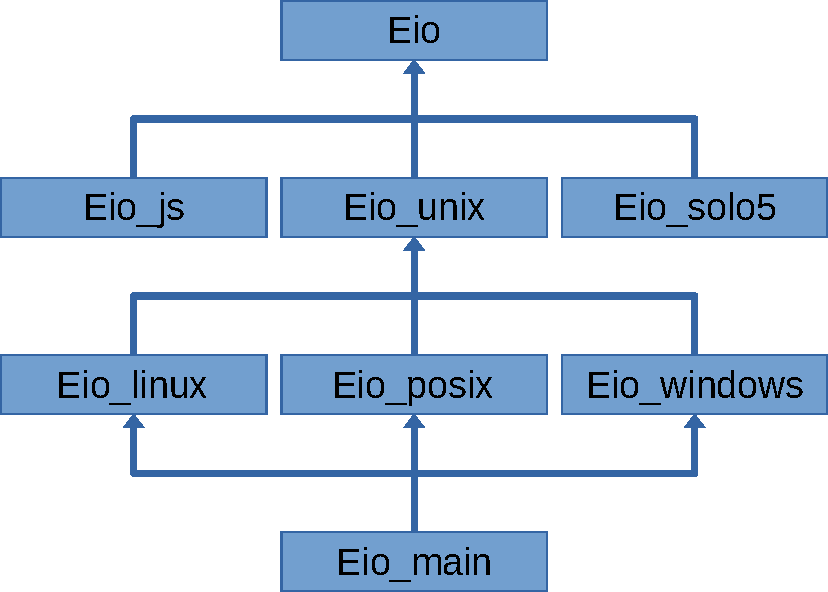
\includegraphics[width=0.6\textwidth]{arch.pdf}
	\end{figure}
\end{frame}

\begin{frame}[fragile]
	\frametitle{Performance : single core}
	\bigskip
	Eio (0.38 s):
\begin{lstlisting}[style=ocaml]
  let parse r =
    for _ = 1 to n_bytes do
      let r = Eio.Buf_read.any_char r in
      ignore (r : char)
    done
\end{lstlisting}
	\bigskip
	Lwt (1.49 s):
\begin{lstlisting}[style=ocaml]
  let parse r =
    let rec aux = function
      | 0 -> Lwt.return_unit
      | i ->
        let* r = Lwt_io.read_char r in
        ignore (r : char);
        aux (i - 1)
    in
    aux n_bytes
\end{lstlisting}
\end{frame}

\begin{frame}
	\frametitle{Performance : multi-core}
	\bigskip
	\begin{itemize}
		\item Many data-structures are now lock-free
		\item Better performance with multiple domains
	\end{itemize}
	\bigskip
	\centering
	Synchronous streams\\
	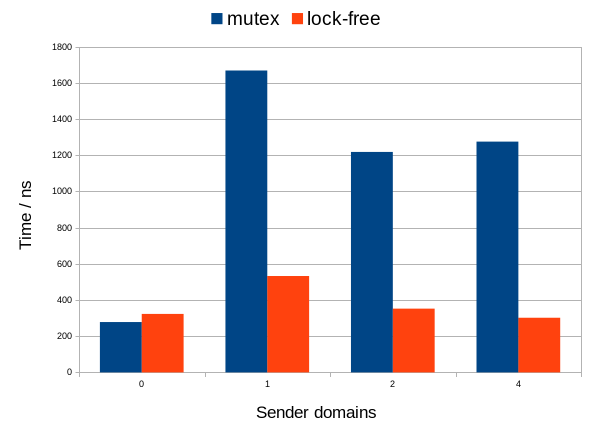
\includegraphics[width=0.8\textwidth]{lock-free.png}
\end{frame}

\begin{frame}[fragile]
	\frametitle{Interoperability : Lwt}
	To run Lwt programs under Eio, replace \verb|Lwt_main.run| with:
\begin{lstlisting}[style=ocaml]
  Eio_main.run @@ fun env ->
  Lwt_eio.with_event_loop ~clock:env#clock @@ fun _ ->
  Lwt_eio.run_lwt @@ fun () ->
  ...
\end{lstlisting}
\verb|run_lwt| and \verb|run_eio| switch between Lwt and Eio code:
\begin{lstlisting}[style=ocaml]
val run_lwt : (unit -> 'a Lwt.t) -> 'a
val run_eio : (unit -> 'a) -> 'a Lwt.t
\end{lstlisting}
	\bigskip
	\url{https://github.com/ocaml-multicore/lwt_eio}
\end{frame}

\begin{frame}[fragile]
	\frametitle{Interoperability : Async}
	\verb|Async_eio| does the same for async:
	\bigskip
\begin{lstlisting}[style=ocaml]
val run_eio :
  (unit -> 'a) -> 'a Async_kernel.Deferred.t

val run_async :
  (unit -> 'a Async_kernel.Deferred.t) -> 'a
\end{lstlisting}
	\bigskip
	\url{https://github.com/talex5/async_eio}
\end{frame}

\begin{frame}[fragile]
	\frametitle{Interoperability : Async, Eio and Lwt}
	You can even use all three libraries together in a single domain!
	\bigskip
\begin{lstlisting}[style=ocaml]
Eio_main.run @@ fun env ->
Lwt_eio.with_event_loop ~clock:env#clock @@ fun _ ->
Async_eio.with_event_loop @@ fun _ ->
...
\end{lstlisting}
	\bigskip
	\url{https://github.com/talex5/async-eio-lwt-chimera}
\end{frame}

\begin{frame}[fragile]
	\frametitle{Interoperability : Domainslib and Kcas}
	Eio, Domainslib and Kcas all use \verb|domain-local-await|,
	allowing e.g. Domainslib to add items to a Kcas queue,
	which is being read from an Eio doman.
\end{frame}


% \begin{frame}
% 	\frametitle{Parsing benchmark}
% 	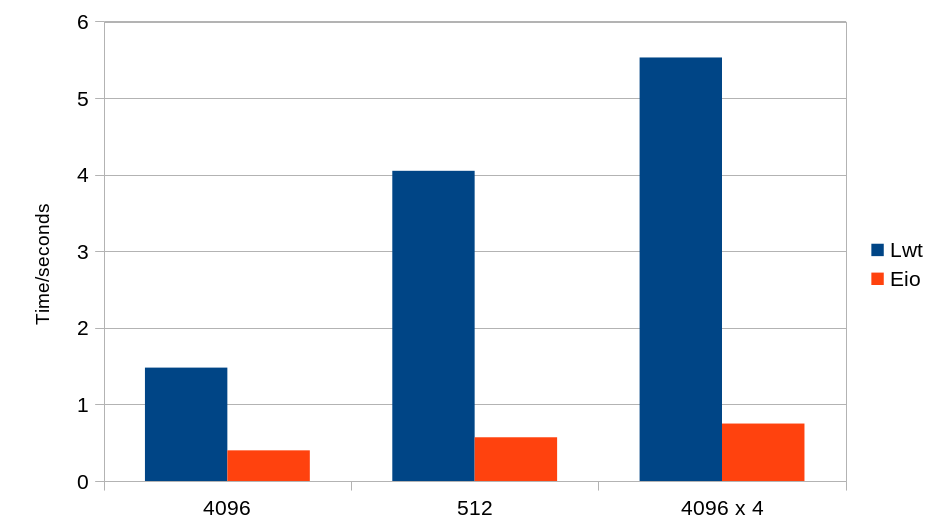
\includegraphics[width=\textwidth]{parsing.png}
% 	Parsing 100,000,000 bytes, one at a time:
% 	\begin{itemize}
% 		\item With a 4096-byte buffer (3.7x faster)
% 		\item With a 512-byte buffer (7.1x faster)
% 		\item With four runs in parallel (7.4x faster)
% 	\end{itemize}
% \end{frame}

\begin{frame}[fragile]
	\frametitle{perf : test code}
\begin{tabular}{ll}
        Eio & Lwt \\
\begin{lstlisting}[style=ocaml,boxpos=t]
  let run_task1 () =
    for _ = 1 to 2000 do
      do_work ()
    done

  let run_task2 () =
    for _ = 1 to 2000 do
      do_work ()
    done

  let run () =
    Fiber.both run_task1 run_task2
\end{lstlisting}&
\begin{lstlisting}[style=ocaml,boxpos=t]
  let run_task1 () =
    let rec outer = function
      | 0 -> Lwt.return_unit
      | i ->
        let* () = do_work () in
        outer (i - 1)
    in
    outer 2000

  let run_task2 () = ...

  let run () =
    Lwt.join [
      run_task1 ();
      run_task2 ();
    ]
\end{lstlisting}
\end{tabular}
\end{frame}

\begin{frame}[fragile]
	\frametitle{perf : results}
        \verb|perf| shows \verb|task1| vs \verb|task2| for Eio part:
	\scriptsize
\begin{verbatim}
- 49.94% Lwt_main.run_495
   - Lwt_main.run_loop_435
      - 49.83% Lwt_sequence.loop_346
         - Lwt.callback_1373
            - 49.77% Dune.exe.Perf.fun_967
               + 49.77% Dune.exe.Perf.use_cpu_273
- 49.90% Eio_linux.Sched.with_sched_inner_3088
   - 49.89% Eio_linux.Sched.with_eventfd_1738
      - Stdlib.Fun.protect_320
         - 49.86% caml_runstack
            - Eio.core.Fiber.fun_1369
               - 25.07% Dune.exe.Perf.run_task2_425
                  + Dune.exe.Perf.use_cpu_273
               - 24.78% Dune.exe.Perf.run_task1_421
                  + 24.77% Dune.exe.Perf.use_cpu_273
\end{verbatim}
\end{frame}

% \begin{frame}[fragile]
% 	\frametitle{Error reporting}
% 	\begin{itemize}
% 		\item Eio takes care to preserve stack-traces
% 		\item \verb|Lwt.join| waits for all threads before reporting errors;
% 		      errors may never be seen
% 		\item \verb|Eio.Fiber.both| cancels the other fiber
% 	\end{itemize}
% 	\bigskip
% 	\begin{lstlisting}[style=ocaml]
% Fiber.both
%   (fun () ->
%      for x = 1 to 1000 do
%        traceln "x = %d" x;
%        Fiber.yield ()
%      done
%   )
%   (fun () -> failwith "Simulated error")
% 
% +x = 1
% Exception: Failure "Simulated error"
% 	\end{lstlisting}
% \end{frame}

\begin{frame}[fragile]
	\frametitle{Resource leaks}
	\begin{itemize}
		\item Resources are attached to switches
		\item When the switch finishes, the resource is freed
	\end{itemize}
	Eio:
	\begin{lstlisting}[style=ocaml]
	let accept socket =
	  Switch.run @@ fun sw ->
	  let conn, _addr = Eio.Net.accept ~sw socket in
	  ...
          Eio.Net.close conn      (* Optional *)
	\end{lstlisting}
        Lwt (leaks \verb|conn| if cancelled):
	\begin{lstlisting}[style=ocaml]
	let accept socket =
	  let* conn, _addr = Lwt_unix.accept socket in
	  ...
	  Lwt_unix.close conn
	\end{lstlisting}
\end{frame}

\begin{frame}[fragile]
	\frametitle{Bounds on behaviour : Lwt}

	\begin{lstlisting}[style=ocaml]
	      let () =
		Lwt_main.run (main ())
	\end{lstlisting}

	\begin{itemize}
		\item What does this program do?
		\item What firewall rules should we set?
		\item Global state is hard to reason about
	\end{itemize}
\end{frame}

\begin{frame}[fragile]
	\frametitle{Bounds on behaviour : Eio}

	\setlength\fboxsep{1.2pt}
	\begin{lstlisting}[style=ocaml,escapechar=!]
let () =
  Eio_main.run @@ fun !\colorbox{highlight}{env}! ->
  Switch.run @@ fun sw ->
  let addr = `Tcp (Eio.Net.Ipaddr.V4.any, 8080) in
  let socket =
    Eio.Net.listen ~sw !\colorbox{highlight}{env}!#net addr
      ~backlog:5
      ~reuse_addr:true
  in
  let dir = Eio.Path.open_dir ~sw (!\colorbox{highlight}{env}!#fs / "/srv/htdocs") in
  main ~socket dir
	\end{lstlisting}
	\begin{itemize}
                \item Listens on port 8080 (no other network use)
                \item Uses \verb|/srv/htdocs| (no other file-system use)
	\end{itemize}
	\bigskip
	\url{https://roscidus.com/blog/blog/2023/04/26/lambda-capabilities/}
\end{frame}

\begin{frame}
	\frametitle{Experiences porting software}
	\begin{itemize}
		\item Solver service (cache-dir bug)
		\item Wayland proxy
		\item Libraries: ocaml-tls, cohttp, dream, capnp-rpc, ...
	\end{itemize}
	\bigskip
	\url{https://github.com/ocaml-multicore/awesome-multicore-ocaml}
\end{frame}

\begin{frame}[fragile]
	\frametitle{Future}
	Eio 1.0:
	\begin{itemize}
		\item Finish file-system APIs
		\item OCaml 5.1 events
	\end{itemize}
	\bigskip
	Get involved:
	\begin{itemize}
		\item Chat on \verb|#eio| (\url{https://matrix.to/#/#eio:roscidus.com})
		\item Developer video call every two weeks
	\end{itemize}
	\bigskip
	\url{https://github.com/ocaml-multicore/eio}
\end{frame}

\end{document}
